%%%%%%%%%%%%%%%%%%%%%%%%%%%%%%%%%%%%%%%%%
%
% In 4073 Embedded Real-Time Systems Course report
% Team 2: Daniel Lemus Perez, Diogo Monteiro and Imara C.T.M. Speek
%
%%%%%%%%%%%%%%%%%%%%%%%%%%%%%%%%%%%%%%%%%

%----------------------------------------------------------------------------------------
%	PACKAGES AND DOCUMENT CONFIGURATIONS
%----------------------------------------------------------------------------------------

\documentclass{article}

\usepackage{graphicx} % Required for the inclusion of images
\usepackage{natbib} % Required to change bibliography style to APA
\usepackage{amsmath} % Required for some math elements 
\usepackage{anysize}
\marginsize{2cm}{2cm}{2cm}{2cm} % decrease the margins

\usepackage{xcolor}
\newcommand\worries[1]{\textcolor{red}{#1}} %add command to specify worries in red
\newcommand\todo[1]{\textcolor{blue}{#1}} % add command to specify todo in blue

\usepackage[toc, page]{appendix} % to include appendices
\usepackage{listings} % to include source code

%\setlength\parindent{0pt} % Removes all indentation from paragraphs

\renewcommand{\labelenumi}{\alph{enumi}.} % Make numbering in the enumerate environment by letter rather than number (e.g. section 6)

%\usepackage{times} % Uncomment to use the Times New Roman font

%----------------------------------------------------------------------------------------
%	DOCUMENT INFORMATION
%----------------------------------------------------------------------------------------

\title{IN4073 Embedded Real-Time Systems \\ QR Lab report - Team II} % Title

\author{Diogo \textsc{Monteiro}, Daniel S. \textsc{Lemus} and Imara C.T.M. \textsc{Speek} \\
		xxxxxx 870754 1506374} % Authors' names

\date{\today} % Date for the report

\begin{document}

\maketitle % Insert the title, author and date

% abstract of 10 lines maximum specifying the specific approach and results
 \begin{abstract}


 \end{abstract}

%----------------------------------------------------------------------------------------
%	INTRODUCTION
%	include the problem statement
%----------------------------------------------------------------------------------------

\section{Introduction}
\label{sec:introduction}


%----------------------------------------------------------------------------------------
%	ARCHITECTURE
%	Specify all software components + interfaces
%----------------------------------------------------------------------------------------

\section{Architecture}
\label{sec:architecture}




%----------------------------------------------------------------------------------------
%	IMPLEMENTATION
%	How you did it and who did what
%----------------------------------------------------------------------------------------

\section{Implementation}
\label{sec:implementation}

This Section introduces the implementation of the functionalities implemented in the system. These concern, GUI communication protocols, safety measures, speed enhancements and basic functionalities.


%-------------------------------------------------------------------------------------------------------------------------------------------------------------------------------------
%GUI
\subsection{GUI}
A simple GUI is designed to control the QR (Figure \ref{fig.GUI}) using QT creator, which allows multi-platform deployment. User can interact with the QR through the keyboard and the GUI (Using the 4 buttons). Buttons functionalities are described in Table \ref{tbl:GUIButts}. \todo{INCLUDE KEYBOARD BUTTONS FUNCTIONALITIES}

\begin{figure}[ht]
\centering
	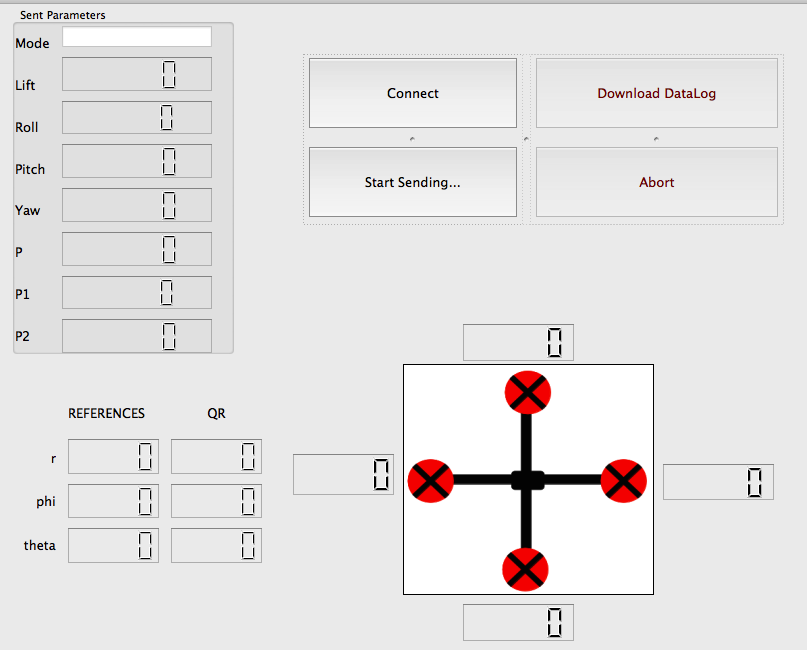
\includegraphics[scale=0.4]{Figures/GUI.png}
	\caption{Designed User Interface}
	\label{fig.GUI}
\end{figure}

\begin{table}[ht]
\centering
\caption{GUI Buttons functionalities}
\begin{tabular}{|c|c|}
\hline 
\textbf{Button} & \textbf{Functionality} \\ 
\hline 
\hline 
Connect / Disconnect & Establishes communication with the QR (through RS232). Once connection is stablished \\ & \emph{Start Sending} button is enabled\\ 
\hline 
Start/Stop Sending & Data is sent and received. Joystick/Keyboard commanded inputs and Telemetry \\ & are displayed   in the display controls. 
\\ & Connect button (Now labelled as Disconnect) is disabled until the \emph{Start/Stop Sending} \\ & button is pressed again.
\\ & \emph{Abort} and \emph{Download DataLog} are enabled
\\
\hline 
Download DataLog & \texttt{EXIT\_MODE} is sent to the QR and data is received and stored in a txt file. 
\\ & \emph{Start/Stop Sending} button is disabled while the data is being stored\\
\hline 
Abort & \texttt{ABORT\_MODE} is sent to the QR making all motor stop immediately\\ 
\hline 
\end{tabular} 
\label{tbl:GUIButts}
\end{table}

Telemetry data are shown in 3 display controls (QR column with r, phi, theta) next to the commanded values (REFERENCES) which are only displayed in \texttt{FULL\_CONTROL} mode.

All commanded signals from the keyboard and joystick are shown in the Lift, Roll, Pitch, Yaw, P, P1, P2 controls as well as the set MODE. P, P2, P3 values are only changed in \texttt{YAW\_CONTROL} and \texttt{FULL\_CONTROL} modes (See \todo{mode selection}).

In addition, four extra controls show the expected motor speed (Along with a QR schematic for easier understanding).

As safety measure, the QR must be set in \texttt{SAFE\_MODE} before communication is stopped (using the \emph{Start/Stop Sending} button). If the user terminates the program, \texttt{SAFE\_MODE} is set in the QR and the RS232 port is closed.

%-------------------------------------------------------------------------------------------------------------------------------------------------------------------------------------
% All info considering communcation protocols
\subsection{Communication Protocols}

%-------------------------------------------------------------------------------------------------------------------------------------------------------------------------------------

\subsubsection{PC-$>$QR}
In order to transmit efficiently data from the PC to the QR, a simple and compact communication protocol was implemented. It consists on a fixed length 7 bytes packet, including a starting byte \textbf{0x80}, 5 parameters and a checksum (Table \ref{tbl:PkgDefinition}). 

\begin{table}[ht]
\centering
\caption{Packet Definition}
\begin{tabular}{|c|c|c|c|c|c|c|}
\hline 
0x80 & MODE & LIFT/- & ROLL/P & PITCH/P1 & YAW/P2 & CHECKSUM \\ 
\hline 
\end{tabular} 
\label{tbl:PkgDefinition}
\end{table}

Although data from the joystick comes in the [$2^{15}$,$2^{15}-1$] range, a single byte is used for each parameter. This is enough taking into account that high sensitivity from the joystick is not needed and rather undesirable (may introduce noise).

The packet structure is composed of
\begin{itemize}

\item{\emph{Starting Byte} \textbf{0x80}, none of the parameters nor the checksum are allowed to have this value.}

\item{\emph{Mode} is set in the second byte as an unsigned char.}

\item{\emph{Lift} is scaled from $[0-255]$ excluding 128 (\textbf{0x80}).}

\item{\emph{Roll}, \emph{pitch} and \emph{yaw} are scaled in the range $[-127,127]$, and then type-cast to unsigned char. The same range is used to scale the control gains (\emph{P} (for yaw control), \emph{P1} and \emph{P2} (for full control)).}

\item{\emph{Checksum} is calculated as a two's complement addition of all parameters (exluding the starting byte). The \textbf{0x80} value is handled and changed to \textbf{0x00}.}

\end{itemize}

The parameters being encapsulated in the packet depend on the selected mode. \emph{Panic, Manual, Calibration,Yaw Control} and \emph{Full Control} modes includes \emph{lift}, \emph{roll},\emph{pitch} and \emph{yaw} as parameters. \emph{P} mode includes 0, \emph{P} (for yaw control), \emph{P1} and \emph{P2} (for full control) gains as parameters (Table \ref{tbl:PkgDefinition}). Although \emph{lift}, \emph{roll},\emph{pitch} and \emph{yaw} are transmitted for safe, panic and calibration modes, they are not acknowledged by the FPGA. Data coming from the joystick and keyboard are scaled in $[0-255]$ range and encapsulated in a single byte (\emph{unsigned char}) per parameter.

A data structure is implemented in the \emph{Package.h} file. This structure includes functions to initialize, set parameters into the packet and calculate the checksum. Some extra functions are included to clip the data to the [-127,127] range and handle with the \textbf{0x80}. This simple communication protocol structure allows the FPGA a more efficiently decoding, handling always with the same packet length.

%-------------------------------------------------------------------------------------------------------------------------------------------------------------------------------------

\subsubsection{Mode selection}
\todo{write about switch case and decoding}
\todo{write about mode selection function in pc}

%-------------------------------------------------------------------------------------------------------------------------------------------------------------------------------------

\subsubsection{Telemetry QR-$>$PC}

Telemetry is used as supervision. It is also used to acknowledge the fpga status (\texttt{TELEMETRY\_FLAG}). Using the retrieved information mode selection is performed in the PC (See. mode selection section ... @Diogo). Along with the FPGA status (\texttt{TELEMETRY\_FLAG}) sensor data is included (yaw rate, pitch and yaw) as follows (Table. \ref{tbl:TelPkgDefinition}). 

\todo{ MENTION HOW FAST THE TELEMETRY IS SENT AND HOW THIS IS PERFORMED IN THE FPGA (WHETHER A ISR IS USED OR NOT)}\\

\todo{mention the internal telemetry (LEDs etc)}

\begin{table}[ht]
\centering
\caption{Telemetry Packet Definition}
\begin{tabular}{|c|c|c|c|c|c|}
\hline 
0x80 & r & phi & theta & TELEMETRY FLAG & CHECKSUM \\
\hline 
\end{tabular} 
\label{tbl:TelPkgDefinition}
\end{table}

Parameter r (yaw rate) is encapsulated in a single byte, whereas phi and theta use 2 bytes each.

%-------------------------------------------------------------------------------------------------------------------------------------------------------------------------------------
% Reliable communication
% 

\subsection{Communication properties}
\subsubsection{Reliability} 
To ensure a \emph{reliable communication} , the sent packets are appended with a checksum.  This checksum is calculated at both the PC and the QR. When the locally calculated checksum does not match the send checksum, the package is regarded as faulty and discarded. The checksum in the \textsc{PC-$>$QR} protocol is calculated using a \emph{two's complement addition checksum} as it has been used before in a previous project by \textbf{Daniel}. The checksum calculation used in the telemetry and data logging written by \textbf{Imara} uses the \textsc{XOR} checksum.  

The two's complement method takes 22 $\mu$s for every addition and requires a complement taking 5 additional $\mu$s while the \textsc{XOR} method takes 22 $\mu$s for every \textsc{XOR}'ing. The \textsc{XOR} checksum has a \emph{Hamming Distance} of 2, detecting all one-bit errors, but not all two-bit errors. This happens when an even number of bit errors occurs in the same bit position of the checksum computational block. The two's complement addition with a Hamming Distance of 2 can be seen as an improvement of the \textsc{XOR} checksum as it mixes between bit positions of the data-blocks as a result of the bit-by-bit carry outs of the additions. As most of the control loop delay is caused by the X32 code, we want to limit the amount of instructions. Because of this and it's data independence we decided to use the \textsc{XOR} checksum 

\subsubsection{Dependability}
Whenever the PC link is broken or disconnected, the code should immediately signal the error and enter panic mode. \textbf{Imara} coded this using a communication counter \texttt{commflag} which is set to zero whenever a package is received in the interrupt service routine of the RS232 RX of the FPGA. Whenever the counter exceeds the threshold \texttt{commthres}, the mode is set to \texttt{PANIC\_MODE}. \todo{explain why this didn't work in the lab}

\subsubsection{Robustness}
\todo{write arithmetic solutions for representing and handling of sensor values, possibly in an image overview?}

%-------------------------------------------------------------------------------------------------------------------------------------------------------------------------------------
% Safety mode, emergency stop, stalling proof, robust to noise, reliable communication, 
% dependability, robustness

\subsection{Safety features}
The \emph{safe mode} is the initial mode in which the QR operates and has to be accessed in between switching modes. \textbf{Imara} coded the safe mode function in the matching header file in which the FPGA's status is updated in the \texttt{telemetry\_flag}. The engine values are decreased using a \texttt{SAFE\_JUMP} value of 5 to avoid stalling of the engines whenever the FPGA operates in safe mode as determined in the \texttt{switch case} in the \texttt{main} function. 

An extra \texttt{abort\_mode} was created by \textbf{Diogo} to distinguish between directly dangerous situations where the FPGA should shut down the engines and shut down and situations where the system can reduce engine values in a controlled manner such as the \texttt{panic\_mode} provides. \todo{Diogo, can you support the reasons for this}

To prevent stalling to occur in the brushless engines, a \texttt{check\_motor\_ramp()} function is called in the PC after the \texttt{mode\_selection()} performs the mode selection. This function written by \textbf{Daniel} clips the ramping up of the engines to a set maximum value for increasing and decreasing of the engine values. This is done by comparing current \texttt{lift} control values with a \texttt{prev\_lift}. 

%-------------------------------------------------------------------------------------------------------------------------------------------------------------------------------------
%   Datalogging
\subsection{Data Logging}

Data logging is used to verify the filtering/controller behaviour, as well as QR behaviour in general. Multiple signals are stored while the QR is running. A 33 bytes packet is stored each 150ms composed by a starting byte (\textbf{0x80}), 16 parameters (31 bytes) and a checksum. Logged data include timestamp (1 byte), MODE, Lift, Roll, Pitch and Yaw (1 byte each), motor commanded speeds (2 bytes each), sensor normalized data (1 byte each) excluding acceleration reading in Z direction, phi and theta angles (2 bytes each), p and q angles (1 byte each), P, P1 and P2 control gains (1 Byte each) and control time (1 byte).

The data is retrieved from the PC once the \emph{exit mode} is triggered (Pressing Del key or clicking in the Data Log button in the GUI). The FPGA exits the while loop and starts sending the stored data. In the mean time the PC stops writing in the port and starts receiving from the fpga. As the data is received, the PC checks for the start byte (\textbf{0x80}) and stores the subsequent bytes until the expected size is reached (33 bytes). Once the complete packet is stored, the checksum is verified and the packet is written into a text file. All packets are separated by a CR and the starting byte is excluded (as the packet is verified before is written into the file).

A matlab script is used to decode and visualize the logged signals.


%-------------------------------------------------------------------------------------------------------------------------------------------------------------------------------------
%   Filtering
\subsection{Filtering}

QR sensor signals must be filtered and bias-cleared before they are feed in the controller. Figure \ref{fig.Noise} shows how signals coming from the accelerometer are noisier than the signals coming from the gyroscopes. Two filter options are explored to perform the signal reconditioning.

\begin{figure}[ht]
\centering
	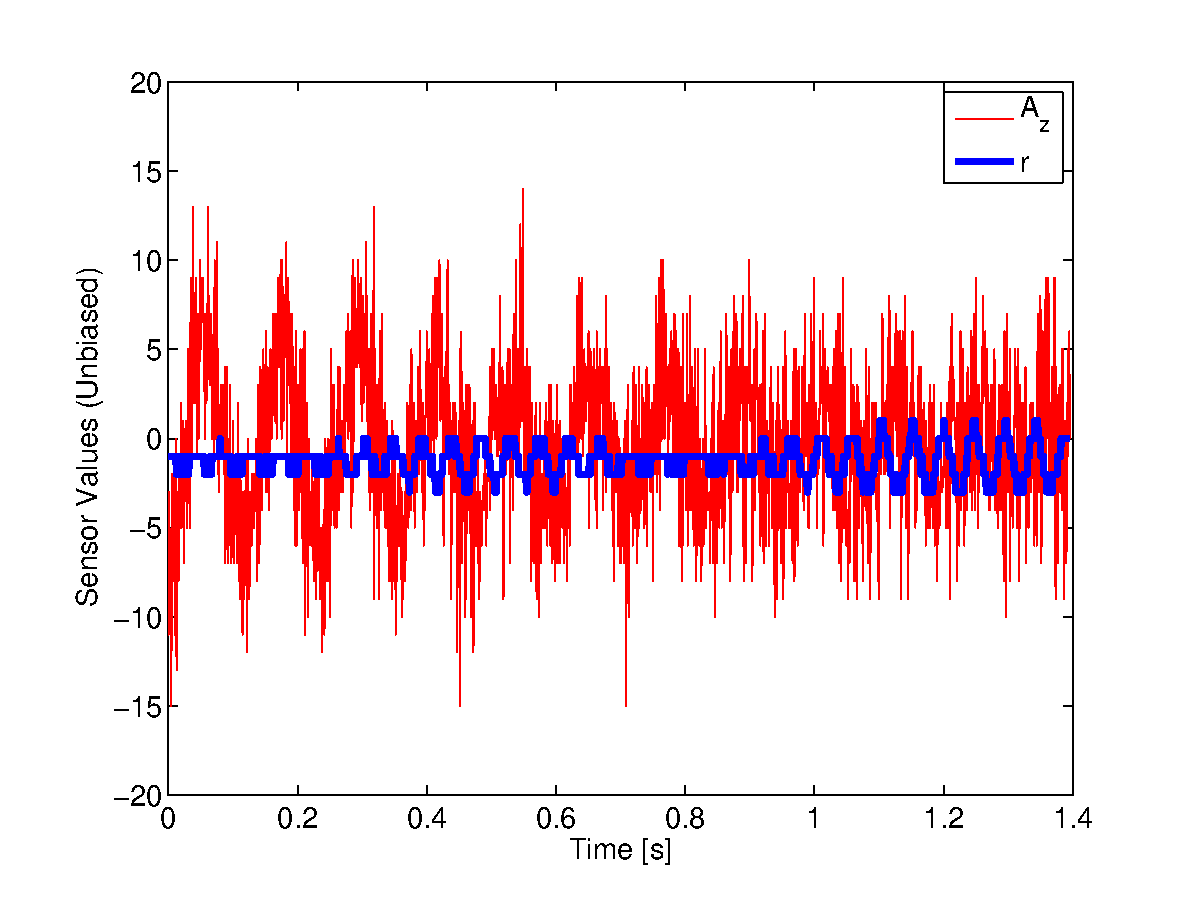
\includegraphics[scale=0.6]{Figures/Noise.eps}
	\caption{Accelerometer vs Gyro noise comparison}
	\label{fig.Noise}
\end{figure}

\subsubsection{Butterworth Filter}

A first order butterworth filter is used to perform noise reduction. This noise reduction can be regulated setting the cutoff frequency. Lower cutoff frequency will lead to a much smoother signal with delay as trade-off. In contrast, higher cutoff frequency results in a synchronised signal with still some noise (Figure \ref{fig.NoiseComp}). Although a lower cut frequency (10Hz) lead to a delayed signal, the phase shift for a butterworth $1^{st}$ order is less than $90^{o}$ at the cut frequency, making it suitable for the QR application. 

\begin{figure}[ht]
\centering
	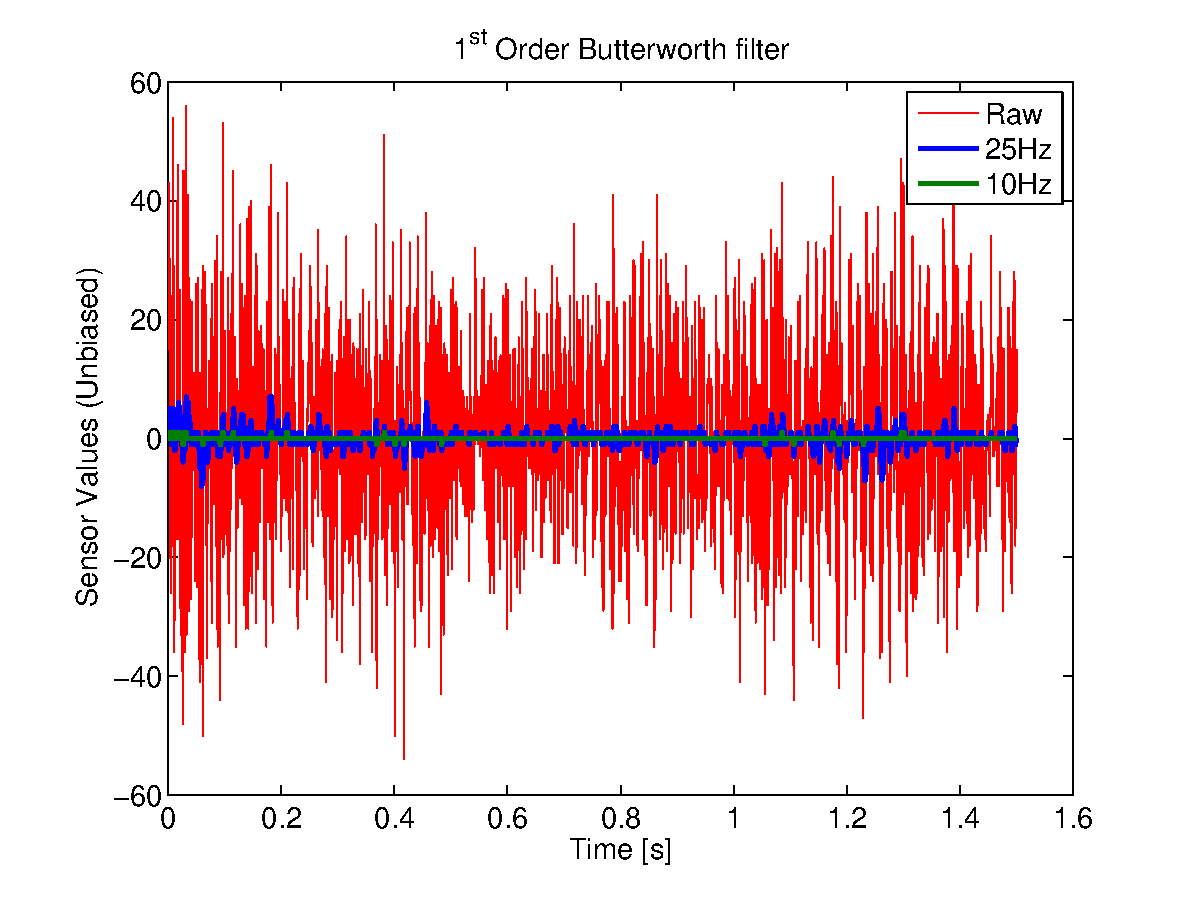
\includegraphics[scale=0.6]{Figures/NoiseComp.eps}
	\caption{Cutoff Frequency effect in a $1^{st}$ order butterworth filter}
	\label{fig.NoiseComp}
\end{figure}

Implementation of a $1^{st}$ order butterworth filter is straightforward. Given the signal sample frequency and the desired cutoff frequency, a set of constants ($A0$,$A1$,$B_0$ and $B_1$) are calculated. Using this constants the filtered signal is reconstructed out from the raw sensor values (current and previous) and the previous filtered value.

\begin{equation}
	 B_0 y_k = A_0 x_k + A_1 x_{k-1} + B_1 y_{k-1}
	 \label{eq:Butt1st}
\end{equation}

where $x$ and $y$ are the raw and filtered values respectively, $A0$,$A1$,$B_0$ and $B_1$ are the constants for a $1^{st}$ order butterworth filter, $k$ and $k-1$ represent the current and previous measurement.

The calculated constants for the $1^{st}$ order butterworth are rational numbers and a proper scaling is applied in order to compute the multiplication with the measured and filtered values (The FPGA soft core does not handle floating point numbers). A 14 bit fix point arithmetic is applied in this case to compute the constants (This is multiply by $2^14$ and round the number as seen in Table \ref{tbl:ButtConstants}).

\begin{table}[ht]
\centering
\caption{Telemetry Packet Definition}
\begin{tabular}{|c|c|c|c|c|}
\hline 
 & $A_0$ & $A_1$ & $B_0$ & $B_1$ \\ 
\hline 
Real Values & 0.0242 & 0.0242 & 1 & -0.9515 \\ 
\hline 
14 Bit Fix Point & 396 & 396 & 16384 & -15590 \\ 
\hline 
\end{tabular}
\label{tbl:ButtConstants}
\end{table}

Once the values are scaled properly multiplication can be computed as the product of two integers dividing the result by $2^14$ (This is made using the $>>$ operator). The outcome of the multiplication is used to compute the filter described in equation \ref{eq:Butt1st}.

\subsubsection{Kalman Filter}






%----------------------------------------------------------------------------------------
%	EXPERIMENTAL RESULTS
%	list the capabilities of your demonstrator
%----------------------------------------------------------------------------------------

\section{Experimental results}
\label{sec:results}



%----------------------------------------------------------------------------------------
%	CONCLUSION
%	Evaluate the design, team results, individual performance and learning experience
%----------------------------------------------------------------------------------------

\section{Conclusion}
\label{sec:conclusion}


%----------------------------------------------------------------------------------------
%	APPENDIX
%----------------------------------------------------------------------------------------

\newpage
\section{Appendices}

\appendix
\section{Title of Appendix A}
\section{Title of Appendix B}



%----------------------------------------------------------------------------------------


\end{document}
